\chapter{Marginal Notes}
Além da área de texto, que normalmente preenche a área de tipo, os documentos geralmente contêm uma coluna para marginália. Você pode definir notas marginais nesta área. Este guia faz uso frequente delas.

\begin{figure}[h]
    \centering
    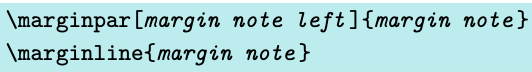
\includegraphics[width=0.6\linewidth]{imagens/imagem25.png}
\end{figure}

As notas marginais no \LaTeX\ são geralmente inseridas com o comando \verb|\marginpar|. Elas são colocadas na margem externa. Documentos de um lado usam a borda direita. Embora você possa especificar uma nota marginal diferente para \verb|\marginpar| caso ela acabe na margem esquerda, as notas marginais são sempre totalmente justificadas. No entanto, a experiência mostrou que muitos usuários preferem notas marginais justificadas à esquerda ou à direita. Para esse propósito, o \KOMAScript\ oferece o comando \char`\\\texttt{mar\-gin\-li\-ne}.

\textbf{Exemplo}: Em algumas partes deste guia, o nome da classe \texttt{scrartcl} pode ser encontrado na margem. Você pode produzir isso com:
\begin{verbatim}
    \marginline{\texttt{scrartcl}}   
\end{verbatim}

Em vez de \verb|\marginline|, você poderia ter usado \char`\\\texttt{mar\-gin\-par}. Na verdade, o primeiro comando é implementado internamente como:
\begin{verbatim}
    \marginpar[\raggedleft\texttt{scrartcl}]
    {\raggedright\texttt{scrartcl}}
\end{verbatim}

Assim, \verb|\marginline| é realmente apenas uma notação abreviada para o código acima.

Usuários avançados encontrarão notas sobre dificuldades que podem surgir usando \char`\\\texttt{mar\-gin\-par} na seção 21.1. Essas observações também se aplicam a \char`\\\texttt{mar\-gin\-li\-ne}. Além disso, o capítulo 19 apresenta um pacote que você pode usar para criar colunas de notas com suas próprias quebras de página.
